\documentclass{my_Presentation}

\title{Agiles Softwaremanagement}
\author{Koch, Merkl, Pfitzner}
\institute{Mobile Robotic Laboratory}
\date{\today}

\begin{document}
%##################################################
\frame{\titlepage \vspace{-0.5cm}
\begin{center}
	\includegraphics[scale=0.5]{Ohm.pdf}\\
	Technische Hochschule N�rnberg
\end{center}
}
%%~~~~~~~~~~~~~~~~~~~~~~~~~~~~~~~~~~~~~~~~~~~~~~~~~~~
\frame{
	\frametitle{Content}
	\begin{minipage}[b]{0.47\linewidth}
		\tableofcontents[pausesection]
	\end{minipage}
		\begin{minipage}[b]{0.47\linewidth}
	\begin{figure}
		\includegraphics[width=\textwidth]{auton.png}
	\end{figure}
%	\begin{figure}
%		\includegraphics[width=\textwidth]{vb_comic.png}
%	\end{figure}
	\end{minipage}
	
}

%%##################################################
\section{Organisation}
\frame{
\frametitle{Teilnehmer}
	\begin{itemize}
		\item \textbf{Stefan May:} Product Owner
		\item \textbf{Philipp Koch:} Scrum Master
		\item \textbf{Christian Merkl:} Teammitglied
		\item \textbf{Christian Pfitzner:} Teammitglied
	\end{itemize}		
	\vfill
	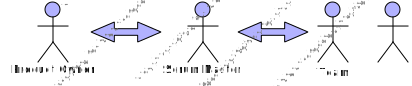
\includegraphics[width=0.9\textwidth]{../grafiken/Team.pdf}
 
}

%%##################################################
\frame{
\frametitle{Zeitplan}
	Gantt Diagramm
}

\section{Das Produkt}
\frame{
\frametitle{Das Produkt}
	\begin{block}{Eine grobe Idee}
		\begin{itemize}
			\item Handy-App
			\item Plattform f�r internationale Studenten
			\item Wichtige Informationen auf einen Blick
			\item Kommunikation untereinander
		\end{itemize}
	\end{block}
	\begin{flushright}
			\includegraphics[width=0.5\textwidth]{../grafiken/s_handy.jpg}
	\end{flushright}
}

%%~~~~~~~~~~~~~~~~~~~~~~~~~~~~~~~~~~~~~~~~~~~~~~~~~~~
\section{Sprint 1}
\frame{
\frametitle{GUI: Programmaufbau}
	\begin{block}{Anforderungen}
		\begin{itemize}
			\item Basisklasse GUI enth�lt m�gliche Designelemente f�r einzelne Abschnitte der APP
			\item Seiten erben von Basisklasse und implementieren eigene Funktionalit�t
		\end{itemize}
	\end{block}
}

\frame{
\frametitle{Gui: Klassendiagramm}
	\begin{center}
			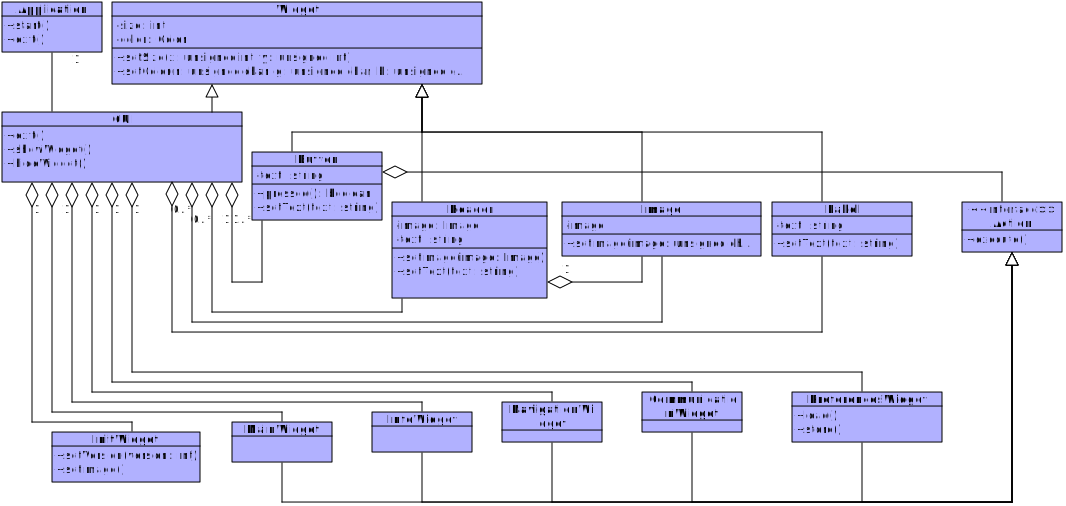
\includegraphics[width=0.9\textwidth]{../grafiken/GUI_Class.pdf}
	\end{center}
}


\frame{
\frametitle{Men�wechsel}
	\begin{block}{Zustandsmaschine}
		\begin{itemize}
			\item Men�punkte werden als Zustand gesehen
			\item zus�tzliche Zust�nde f�r Start und Beenden der Application
			\item Zust�nde k�nnen wiederum Unter-Zust�nde besitzen
		\end{itemize}
		\begin{center}
			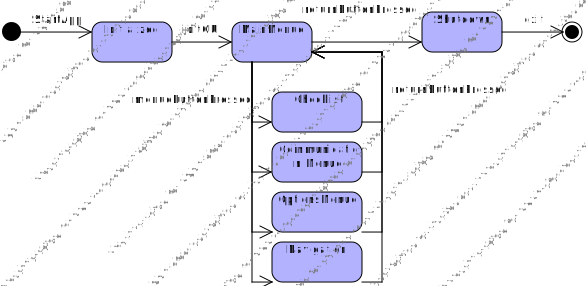
\includegraphics[width=0.8\textwidth]{../grafiken/MenueStates.pdf}
		\end{center}
	\end{block}
}




%%##################################################
\section{Sprint 2}
\subsection*{Datenhaltung: Backend}
\frame{
\frametitle{Hochschulkommunikation}
	\begin{block}{Kommunikation mit Hochschul-Content}
		\begin{itemize}
			\item Hochschule interne Daten �ber Content System
			\item Content-Zugriff bei Internetzugriff des Mobilfunktger�ts
		\end{itemize}
		\includegraphics[width=0.9\textwidth]{../grafiken/OhmCollab.pdf}
	\end{block}
}

\frame{
\frametitle{Datenhaltung}
	\begin{block} {Content Management System (CMS)}
	\begin{itemize}
		\item CMS zum Verwalten von Inhalten
		\item Verschiedene Benutzerrollen:	
			\begin{itemize}
				\item Administrator: Bearbeitung von Design und Inhalt
				\item Redakteuer: Bearbeitung von Inhalt
			\end{itemize}
		\item $\rightarrow$ Hochschule benutzt bereits CMS Systeme f�r Inhalte der Webseite. \\\textbf{Vorteil: zus�tzliche Schulung nicht notwendig} 
	\end{itemize}
	\end{block}
	\begin{block} {Datenbank}
	\begin{itemize}
		\item mySQL-Datenbank	
		\item zyklisches Aktualisieren auf Endanwendung
	\end{itemize}
	\end{block}
}

\frame{
\frametitle{Zusammenspiel}
	\begin{block}{Diagramm}
		\includegraphics[width=1.0\textwidth]{../grafiken/DB.pdf}
	\end{block}
}

\subsection*{Navigation}
\frame{
\frametitle{Navigation: Struktur}
	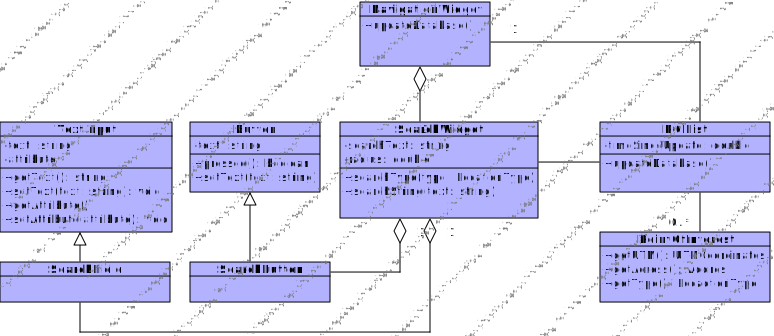
\includegraphics[width=0.9\textwidth]{../grafiken/NavigationW_Class.pdf}
}

\frame{
\frametitle{Interessantes}
	\begin{block}{Struktur}
	\begin{itemize}
		\item Basisklasse f�r interessante Objekte 
		\item Addressinformation f�r schnelles finden von Orten in der Umgebung
		\item UTM-Koordinaten zur �bergabe an Routenplanner
	\end{itemize}
	\begin{center}
		\includegraphics[width=0.8\textwidth]{../grafiken/PointOfInteresst.pdf}
	\end{center}
	\end{block}
}

%%##################################################


\section{Sprint3}

\section{Sprint4}

%%##################################################
\section{Ablauf}
\subsection*{Sprint 1}
\frame{
\frametitle{Sprint 1 - Hauptmenu}
  \begin{block}{Extraktion aus Product Backlog}
   \begin{itemize}
   \item Design des Hauptmenu
    \item Design des Startbildes
    \item Implementierung der Grundfunktionalitaet (Dummy-Funktionen)
    \end{itemize}
  \end{block}  

}

%%##################################################

\subsection*{Sprint 2}
\frame{
\frametitle{Sprint 2 - Kartenwidgets}
  \begin{block}{Extraktion aus Product Backlog}
    \begin{itemize}
    \item Lageplan der TH integrieren
    \item Google-maps plugin implementieren
    \item Implementierung interaktiver Liste fuer Kartenwidgets
    \item Darstellen von Orten aus der Liste in der Karte
    \end{itemize}
  \end{block}  

}

%%##################################################

\subsection*{Sprint 3}
\frame{
\frametitle{Sprint 3 - Kommunikation}
  \begin{block}{Extraktion aus Product Backlog}
    \begin{itemize}
    \item Schnittstelle zu TH-Email / Kalender implementieren
    \item Reminder in Statusleiste implementieren
    \item Popup fuer akute Termine implementieren 
    \item Implementierung des Checklistenwidgets
    \item Design des Reminders erstellen
    \item Design des Popups erstellen
    \item Design des Checklistenwidgets erstellen
    \end{itemize}
  \end{block}  

}

%%##################################################

\subsection*{Sprint 4}
\frame{
\frametitle{Sprint 4 - Redesign}
  \begin{block}{Entscheidung des PO - Name der Hochschule wurde ge?ndert}
  \end{block}
  \begin{block}{Extraktion aus Product Backlog}
    \begin{itemize}
    \item Aenderung der Logos in allen Widgets
    \item Aenderung der TH-Schriftzuege in allen Widgets
    \item Redesign des Startbildschirms
    \end{itemize}
  \end{block}  
  
}

%%################################################## 

\section{Fazit}
\frame{
\frametitle{Lessons Learned}
	\begin{block}{Was lief gut?}
		\begin{itemize}
			\item erster Punkt
		\end{itemize}
	\end{block}
	\begin{block}{Was lief schlecht?}
		\begin{itemize}
			\item erster Punkt
		\end{itemize}
	\end{block}
}

%%~~~~~~~~~~~~~~~~~~~~~~~~~~~~~~~~~~~~~~~~~~~~~~~~~~~
\frame{
\frametitle{Thank you for your attention}
	\begin{block}{Contact}
	\flushright{
	\tiny Title.\\ \normalsize
	\textbf{Name} \\
	Laboratory of mobile Robotics\\
	Kesslerplatz 12 -- KA 640\\
	90489 Nuremberg \\
	\url{Email40432@ohm-hochschule.de}
	}
	\end{block}	
	\begin{figure}
		\includegraphics[width=0.5\textwidth]{auton.png}
	\end{figure}
}

%##################################################
\frame{%\section*{References}
\frametitle{References}
	\begin{block}{Verwendete Software}
			\begin{itemize}
				\item Eclipse Kepler 
				\item Visual Paradigm for UML Professional Edition
			\end{itemize}
	\end{block} 
		
	References

}
\end{document}
